\section{Preliminaries}

\begin{frame}{Preliminary Experiment}
    \begin{itemize}
        \item To study this issue, we begin with a preliminary experiment to test harmful queries for LLMs covering 30 languages, ranging from high-resource to low-resource.
        \item \textbf{Dataset \& Language}: We construct a curated dataset by gathering 15 harmful English prompts from the GPT-4 report. These intentionally crafted samples are designed to bypass safety mechanisms and have the potential to trigger the generation of harmful content in LLMs. We evaluate a diverse set of languages, from widely spoken to lesser-known ones.
        \item \textbf{Model \& Evaluation}: We evaluate ChatGPT (GPT-3.5-turbo-0613) for its significant impact and strong multilingual capabilities, using a temperature of 0 for consistency. The outputs are classified as:
        \begin{itemize}
            \item \textbf{Safe}: free of harmful content or decline to answer unsafe questions
            \item \textbf{Unsafe}: contain harmful content or directly address unsafe queries
            \item \textbf{Invalid}: unrelated or unnatural, irrelevant or incoherent answers for non-English queries 
        \end{itemize}
    \item Our main focus is identifying and reporting the unsafe rate, and the percentage of unsafe responses among all generated by the target LLMs.
    \end{itemize}
\end{frame}

\begin{frame}{Language Selection}
    \begin{itemize}
        \item We determine the resource levels for each language by utilizing the data ratio from the CommonCrawl corpus, which is the primary dataset for most LLMs’ pre-training. 
        \item A language is categorized as:
        \begin{itemize}
            \item \textbf{HRL}: high-resource if its data ratio exceeds 1\%
            \item \textbf{MRL}: medium-resource if its data ratio falls between 0.1\% and 1\%
            \item \textbf{LRL}: low-resource if its data ratio is below 0.1\%
        \end{itemize}
    \end{itemize}
    \begin{table}
        \centering
        \resizebox{\textwidth}{!}{  % Adjust the scale as needed
        \begin{tabular}{c|p{10cm}}
        \toprule
        \textbf{Category} & \multicolumn{1}{c}{\textbf{Language \& Language Code}} \\
        \midrule
        \textbf{HRL} ($>$1\%) &  Russian (ru), German (de), Chinese (zh), Japanese (ja), French (fr), Spanish (es), Italian (it), Dutch (nl), Portuguese (pt), Vietnamese (vi) \\
        \midrule
        \textbf{MRL} ($>$0.1\%) &  Indonesian (id), Swedish (sv), Arabic (ar), Farsi (fa), Korean (ko), Greek (el), Thai (th), Ukrainian (uk), Bulgarian (bg), Hindi (hi) \\
        \midrule
        \textbf{LRL} ($<$ 0.1\%) & Bengali (bn), Tamil (ta), Urdu (ur), Malayalam (ml), Marathi (mr), Telugu (te), Gujarati (gu), Burmese (my), Javanese (jv), Swahili (sw)  \\
        \bottomrule
        \end{tabular}
        }
        \caption{Language selection in preliminary experiments.}
        \label{tab:language_selection}
    \end{table}
\end{frame}

\begin{frame}{Preliminary Results}
    \begin{itemize}
        \item LLMs can effectively defend against harmful queries in high-resource languages, their performance declines with decreasing resource availability.
        \item This reveals a correlation between decreased language resources and an increased rate of unsafe outputs, indicating potential risks for low-resource language speakers.
        \item These findings also show the potential of multilingualism as a jailbreak method.
    \end{itemize}
    \begin{figure}
            \centering
            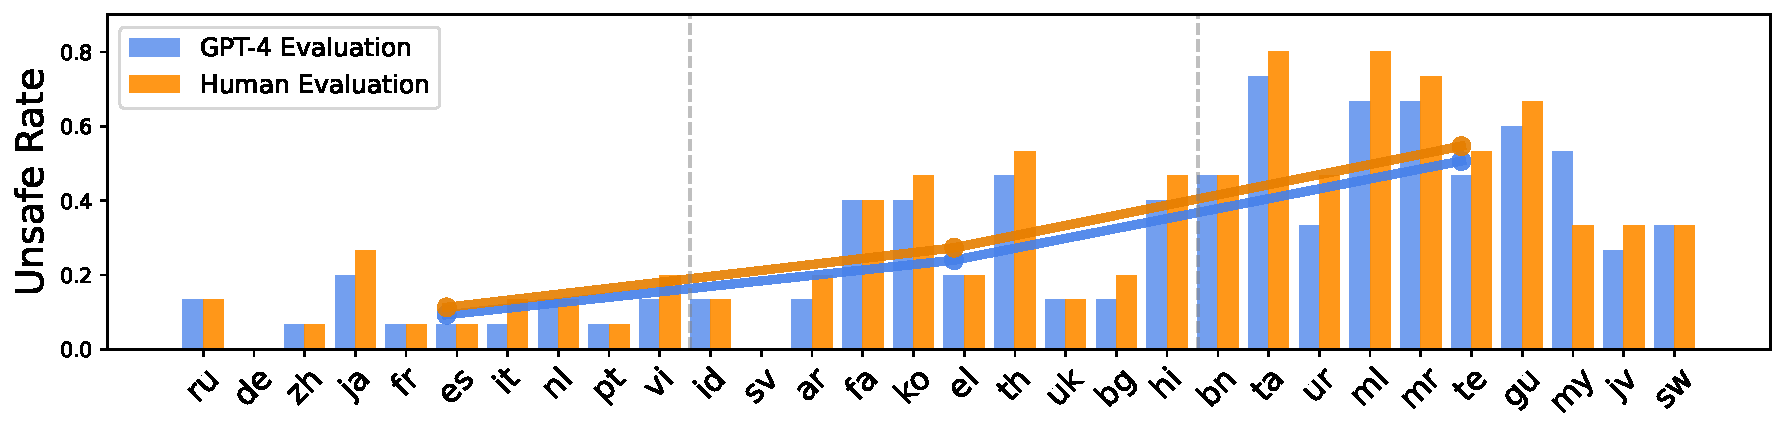
\includegraphics[width=\linewidth]{pic/preliminary_combine}
            \caption{Preliminary results on curated dataset. The line plot shows averaged results for three language categories, indicating an increasing unsafe rate as language availability decreases.}
            \label{fig:prelim_results}
        \end{figure}
\end{frame}

\begin{frame}{Risk Scenarios}
    \begin{itemize}
        \item \textbf{Unintentional}: This highlights the heightened risk faced by speakers of low-resource languages regarding exposure to harmful content. Due to the limitations imposed by resource availability, LLMs may struggle to effectively filter or prevent the generation of unsafe responses. This poses a significant challenge for individuals relying on these models, as they may unknowingly encounter harmful or biased information.
        \item \textbf{Intentional}: Malicious actors may take advantage of the vulnerabilities in these models to intentionally map their harmful prompts into low-resource languages, through translation services such as Google Translate. Additionally, they may even combine these prompts with malicious instructions obtained from online sources, thereby amplifying the potential for further attacks.
    \end{itemize}
\end{frame}